\documentclass[9pt,twocolumn,twoside,lineno]{pnas-new}

%% Some pieces required from the pandoc template
\providecommand{\tightlist}{%
  \setlength{\itemsep}{0pt}\setlength{\parskip}{0pt}}

% Use the lineno option to display guide line numbers if required.
% Note that the use of elements such as single-column equations
% may affect the guide line number alignment.


\usepackage[T1]{fontenc}
\usepackage[utf8]{inputenc}


\templatetype{pnasresearcharticle}  % Choose template

\title{Race-based disparities in academic disciplinary actions are associated
with county-level rates of racial bias}

\author[a]{Travis Riddle}
\author[a,b]{Stacey Sinclair}

  \affil[a]{Princeton University, Department of Psychology, Princeton, NJ, 08544}
  \affil[b]{African American Studies}


% Please give the surname of the lead author for the running footer
\leadauthor{Riddle}

% Please add here a significance statement to explain the relevance of your work
\significancestatement{Black students in the United States are subject to disciplinary action
at rates much higher than their white counterparts. These disciplinary
actions put students at higher risk for negative life outcomes,
including involvement in the criminal justice system. Using government
data covering over 32 million students at nearly 93k schools, our
research demonstrates that the disciplinary gap between black and white
students across 5 different types of disciplinary actions is associated
with county-level rates of explicit racial bias, and suggests solving
racial disparities in education must involve combating explicit racial
bias.}


\authorcontributions{TR and SS designed the research and wrote the paper. TR analyzed the
data.}

\authordeclaration{Authors have no known conflicts of interest}


\correspondingauthor{\textsuperscript{} }

% Keywords are not mandatory, but authors are strongly encouraged to provide them. If provided, please include two to five keywords, separated by the pipe symbol, e.g:
 \keywords{  one |  two |  optional |  optional |  optional   }

\begin{abstract}
There are substantial gaps in academic achievement between black and
white students in the United States. Recently, increased attention has
focused on differences in the rates at which black and white students
are disciplined, finding that black students are more likely to be seen
as problematic and more likely to be punished than white students are
for the same offense. Although these disparities suggest that racial
biases are a contributor, no previous research has shown associations
with psychological measurements of bias and disciplinary outcomes. We
show that county-level estimates of explicit racial bias, as measured
using data from approximately 1.3 million visitors to the Project
Implicit website, are associated with racial disciplinary disparities
across approximately 93k schools in the United States, covering around
32 million white and black students. These associations do not extend to
explicit or implicit sexuality biases, showing the specificity of the
effect. These findings suggest that reducing racial disparities in
education may require efforts to reduce explicit racial bias.
\end{abstract}

\dates{This manuscript was compiled on \today}
\doi{\url{www.pnas.org/cgi/doi/10.1073/pnas.XXXXXXXXXX}}

\begin{document}

% Optional adjustment to line up main text (after abstract) of first page with line numbers, when using both lineno and twocolumn options.
% You should only change this length when you've finalised the article contents.
\verticaladjustment{-2pt}

\maketitle
\thispagestyle{firststyle}
\ifthenelse{\boolean{shortarticle}}{\ifthenelse{\boolean{singlecolumn}}{\abscontentformatted}{\abscontent}}{}

% If your first paragraph (i.e. with the \dropcap) contains a list environment (quote, quotation, theorem, definition, enumerate, itemize...), the line after the list may have some extra indentation. If this is the case, add \parshape=0 to the end of the list environment.

\acknow{Please include your acknowledgments here, set in a single paragraph.
Please do not include any acknowledgments in the Supporting Information,
or anywhere else in the manuscript.}

In comparison to White Americans, Black Americans exhibit poorer
educational outcomes across a range of metrics. One outcome of
particular concern is the gap in disciplinary actions (1, 2). Research
using administrative datasets and longitudinal samples clearly show that
Black American students are far more likely to be suspended or expelled
(3, 4), and conditional on an office referral, are more likely to
receive stiffer punishments (5, 6). These disparities are particularly
concerning as they are associated with long-term life outcomes,
including prospects for employment (7) and involvement in the criminal
justice system (8).

As complex social phenomena, these racial differences in disciplinary
outcomes are multiply determined (2). There are clear structural and
socieconomic contributors such as the practice of segregating students
into achievement-based ``tracks'' of low and high performers (9) or
racial differences in socioeconomic status (10). However, racial bias is
also thought to contribute to the problem. For instance, in a controlled
study, (11) found that in comparison to white students, teachers were
more likely to view the same behavior from black students as being
indicative of a long term problem and deserving of suspension.
Similarly, using discipline data from an urban high school, (12) showed
that black students were especially likely to be referred to the office
for disciplinary action on the basis of defiant behavior - a relatively
subjective category of misbehavior in comparison to others they
examined, including truancy or fighting. Overall, there has been
consistent evidence that black students' behaviors are both perceived as
more problematic and are punished more harshly as compared to white
students'. However, to our knowledge, there has been no work assessing
whether racial bias is directly associated with disciplinary
disparities. Additionally, there has been no work assessing how racial
bias at the community level is associated with educational disparities.

Psychological measurements of racial bias typically occur through one of
two ways. Either individuals are asked to self-report their relative
attitudes toward different racial groups, or via methods designed to
assess automatic associations with people of different races. The latter
is thought to reflect the associations learned by early and frequent
exposure to environmental stimuli, whereas the former reflects top-down
modulation of those associations (13). Recently, researchers have begun
aggregating these measures up to geographical regions such as counties
or states, finding that regional-level measures of implicit and explicit
racial bias are associated with racial disparities in key social
outcomes, although the relative contributions are not consistent across
studies (14--16). For example, (14) found that Black Americans had
reduced access to health care and increased rates of death due to
circulatory disease in comparison to whites in counties with higher
levels of explicit racial bias against blacks. They found no such
associations for implicit racial bias. In contrast, (16), found that the
disproportionate use of lethal force by police on Black Americans was
associated with regional implicit biases, but were not associated with
explicit biases. As such, it is important to assess both types of bias
when seeking to understand the relationship between regional-level bias
and behavioral outcomes.

Regional levels of bias could be associated with the size of racial
student disciplinary disparities for a number of reasons. First, being
in an area characterized by higher racial bias likely means encountering
individuals who have negative feelings and beliefs about one's group.
The actions of such individuals within and/or outside of an educational
setting could contribute to disciplinary disparities. For example, if
teachers and administrators are biased, then they may be more likely to
make decisions that are unfavorable to black students, such as deciding
that a given misbehavior is worthy of official disciplinary action.
Biased administrators or local voters might also support school or
district policies thought to disproportionally punish students of color,
such as zero-tolerance policies or implementation of random drug sweeps
(17). Second, Black students who live in high bias areas may be more apt
to engage in behavior that warrants disciplinary action due to behavior
confirmation of the negative expectancies held by area peers and adults
(18--20). Third, the norms and structural factors (e.g., laws, policies)
that characterize regions higher in bias may constrain even those
individuals who are not biased themselves into engaging in or suborning
actions that negatively impact students of color (21, 22). Fourth,
biases assessed at the regional level might reflect affordances of the
local environment (e.g., confederate statues, biased media) that
undergird these biases and prime behaviors that contribute to
disciplinary disparities (23). Overall, these reasons, and the likely
possibility that they work in concert to inform behavior (24),
substantiate the possibility that there will be a relationship between
regional bias and disciplinary outcomes.

Most previous research has focused on out-of-school suspensions - likely
because they are the most frequently used and are regularly found to be
associated with negative outcomes (25, 26). However, other disciplinary
outcomes, though used less often, may be at least as damaging to
students as out-of-school suspensions (27). For instance school arrests
have been associated with increased likelihood of engaging in
anti-social behavior (28), and with increased risk of dropping out (8).
In addition, though alternative forms of discipline (e.g., in-school
suspension) are intended to insulate students from the negative
consequences of exclusionary discipline, the criteria by which students
are assigned the former kind of discipline often remain vulnerable to
bias (29). As such, examining the presence and basis of disparities in
the application of a wide range of disciplinary actions is warranted.

The present analyses combine regionally-coded implicit and explicit
racial bias measures from approximately 1.3 million respondents who
visited Project Implicit (30) with the most recent available data from
the Civil Rights Data Collection (CRDC) conducted by the US Department
of Education, a mandated census of disciplinary action in all US public
k-12 schools. The CRDC allowed well-powered examinations of five
different disciplinary metrics: in-school suspensions, out-of-school
suspensions, law enforcement referrals, school-related arrests, and
expulsions. We designed the analyses to determine whether, and if so the
extent to which regional estimates of pro-White/anti-Black implicit and
explicit bias are associated with black-white outcomes in disciplinary
gaps. We also use regional estimates of sexuality bias from Project
Implicit to determine whether demonstrated patterns are distinct to
racial bias, or an epiphenomenal associate of bias measures in general.

\subsection{Results}\label{results}

\subsubsection{Project Implicit
estimates}\label{project-implicit-estimates}

We first report the results of estimating the implicit and explicit
biases from Project Implicit data. When examining the unstandardized
county-level estimates adjusted with poststratification, we see that
there is a pro-white bias in both implicit (\(mean\) = 0.4, \(sd\) =
0.02) and explicit measures (\(mean\) = 0.83, \(sd\) = 0.17), where on
both scales 0 = no bias, and positive numbers indicate a pro-white bias.

\subsection{Disciplinary action
frequency}\label{disciplinary-action-frequency}

\begin{table}[!htbp] \centering 
  \caption{Percentage of students of each race receiving each type of disciplinary action} 
  \label{tab:disc-count} 
\begin{tabular}{@{\extracolsep{5pt}} ccc} 
\\[-1.8ex]\hline 
\hline \\[-1.8ex] 
metric & black & white \\ 
\hline \\[-1.8ex] 
school arrests & 0.29\% & 0.09\% \\ 
expulsions & 0.48\% & 0.22\% \\ 
law enforcement referral & 0.75\% & 0.34\% \\ 
in-school suspension & 11.11\% & 4.23\% \\ 
out-of-school suspension & 13.87\% & 3.63\% \\ 
\hline \\[-1.8ex] 
\end{tabular} 
\end{table}

Table \ref{tab:disc-count} shows the percentage of students of each race
who were reported having received each of the actions under
consideration. Additionally, figure \ref{fig:suspension-disp-map} shows
the relative risk ratio for out-of-school suspensions across counties.
Our statistical models (described below) show that the racial
differences seen here are extremely unlikely to be due to chance.

\begin{figure}
\centering
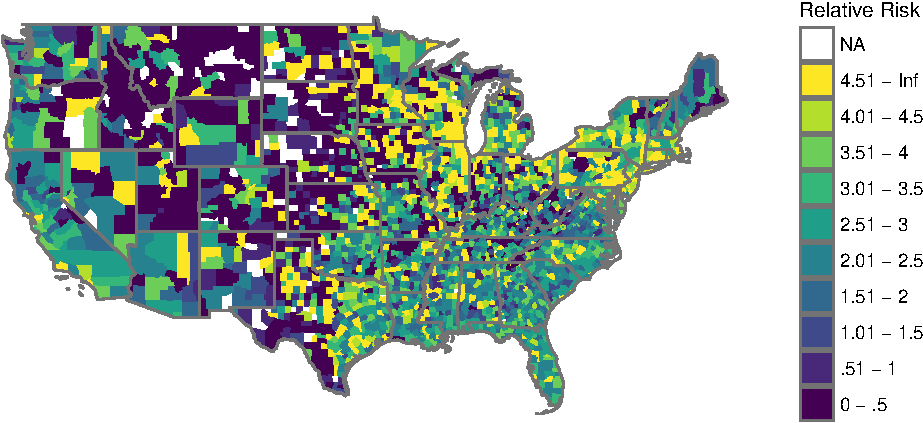
\includegraphics{Riddle_Sinclair_PNAS_files/figure-latex/suspension-disp-map-1.pdf}
\caption{Relative Risk Ratio for out-of-school suspensions for each
county in the continental United States. Relative risk ratio is computed
as the percentage of black students suspended to the percentage of white
students suspended, as reported in the CRDC. Higher values indicate more
black students suspended, relative to white students. Counties with the
value NA either have no schools, have zero black students enrolled, or
have zero white students enrolled. Interactive maps for all disciplinary
outcomes and bias estimates can be found at \url{https://osf.io/pu79a/}}
\end{figure}

\subsection{Associations across
counties}\label{associations-across-counties}

Figure \[fig:overall-associations\] shows the estimate of primary
interest for each of the models. The estimates displayed are the
coefficients for the interaction between race and each of the two bias
measurements. Given that Black Americans are the baseline group,
negative values for this coefficient indicate that as one moves into
counties with higher levels of bias, the gap between the probability of
a black student being disciplined and the probability of a white student
being disciplined grows. Table \[tab:reg-coefs\] displays the estimated
coefficients and 95\% uncertainty intervals for each of the fixed
effects for each model.

\begin{figure}
\centering
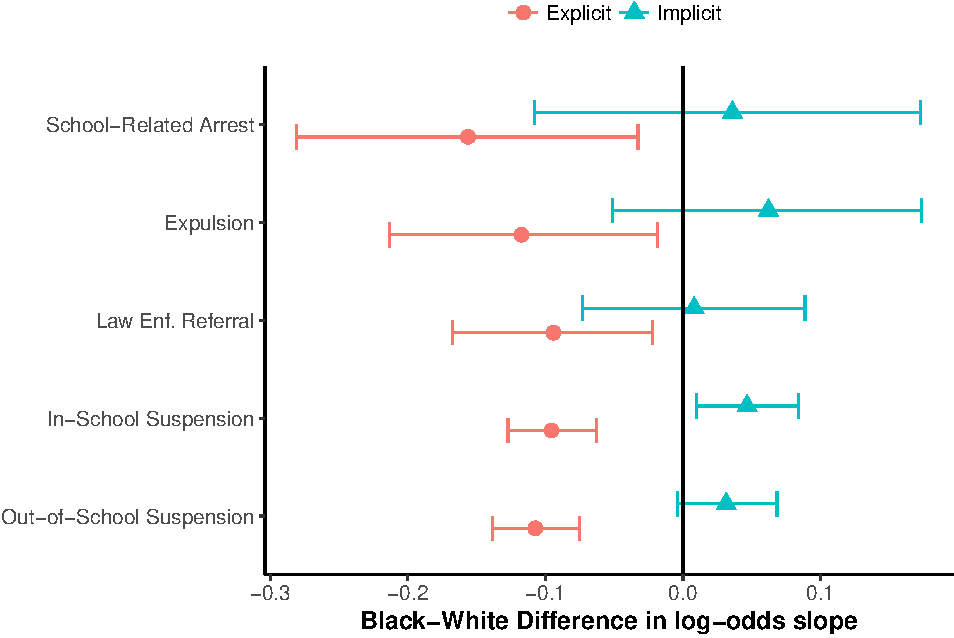
\includegraphics{Riddle_Sinclair_PNAS_files/figure-latex/overall-associations-1.pdf}
\caption{Association between each metric and county-level estimates of
explicit and implicit bias. Negative values indicate that the rate of
increase (or decrease) for blacks is faster (or slower) than for whites.
Point is the mean of the posterior and error bars represent 95\%
bayesian uncertainty intervals}
\end{figure}

Several patterns are apparent from this figure. First, county-level
explicit biases are reliably associated with disciplinary disparities,
such that counties with more bias are expected to have a larger racial
gap. The effect with the largest magnitude of these is school-related
arrests (\(M_{slope}\) = -0.16, {[}-0.28, -0.03{]}), followed by
expulsions (\(M_{slope}\) = -0.12, {[}-0.21, -0.02{]}), out-of-school
suspensions (\(M_{slope}\) = -0.11, {[}-0.14, -0.08{]}), in-school
suspensions (\(M_{slope}\) = -0.1, {[}-0.13, -0.06{]}), and law
enforcement referrals (\(M_{slope}\) = -0.09, {[}-0.17, -0.02{]}).

In contrast, the estimated effects for implicit bias are more ambiguous.
Expulsions (\(M_{slope}\) = 0.06, {[}-0.05, 0.17{]}), school-related
arrests (\(M_{slope}\) = 0.04, {[}-0.11, 0.17{]}), and law enforcement
referrals (\(M_{slope}\) = 0.01, {[}-0.07, 0.09{]}) are all estimated to
be close to zero, or with substantial uncertainty with respect to the
direction of the effect. Surprisingly, there is a reliable association
for in-school suspensions, with schools higher in implicit bias having
smaller in-school suspension gap (\(M_{slope}\) = 0.05, {[}0.01,
0.08{]}). Though not fully conclusive, the the association between
implicit biases and out-of-school suspensions tends to be in a similar,
counter-intuitive direction (\(M_{slope}\) = 0.03, {[}0, 0.07{]}).
However, it is important to point out that at no point do these
associations ``cross over'' such that white students are actually
suspended more frequently than black students. Even at a county with
implicit bias 3 standard deviations above the mean, for every white
student who receives an out-of-school suspension, about 2.43 {[}2.2,
2.66{]} black students are expected to be suspended.

\begin{table}[!htbp] \centering 
  \caption{Regression coefficient estimates for the population-level (i.e. fixed) effects, along with 95\% uncertainty intervals for each of the disciplinary metrics.} 
  \label{tab:reg-coefs} 
\begin{tabular}{@{\extracolsep{5pt}} cccccc} 
\\[-1.8ex]\hline 
\hline \\[-1.8ex] 
 & Out-of-School Suspension & In-School Suspension & Law Enf. Referral & Expulsion & School-Related Arrest \\ 
\hline \\[-1.8ex] 
Intercept & \textbackslash bf\{-2.31\}, [-2.34,-2.28] & \textbackslash bf\{-2.23\}, [-2.27,-2.2] & \textbackslash bf\{-5.77\}, [-5.87,-5.67] & \textbackslash bf\{-6.54\}, [-6.66,-6.42] & \textbackslash bf\{-7.97\}, [-8.18,-7.77] \\ 
black-white ratio & \textbackslash bf\{-0.15\}, [-0.21,-0.1] & \textbackslash bf\{-0.32\}, [-0.4,-0.24] & 0.13, [-0.04,0.29] & -0.09, [-0.29,0.12] & 0.16, [-0.18,0.48] \\ 
proportion black & \textbackslash bf\{0.22\}, [0.13,0.31] & \textbackslash bf\{0.16\}, [0.05,0.28] & \textbackslash bf\{-0.36\}, [-0.6,-0.12] & -0.23, [-0.52,0.07] & -0.37, [-0.79,0.07] \\ 
college grads & \textbackslash bf\{0.08\}, [0.04,0.12] & \textbackslash bf\{-0.06\}, [-0.1,-0.01] & \textbackslash bf\{0.15\}, [0.05,0.26] & -0.03, [-0.16,0.1] & \textbackslash bf\{0.22\}, [0.04,0.41] \\ 
crime & \textbackslash bf\{0.04\}, [0.01,0.07] & \textbackslash bf\{0.05\}, [0.01,0.09] & 0.04, [-0.05,0.12] & \textbackslash bf\{0.12\}, [0.03,0.22] & 0.02, [-0.13,0.16] \\ 
housing density & \textbackslash bf\{-0.05\}, [-0.07,-0.02] & -0.03, [-0.07,0] & 0.01, [-0.06,0.08] & -0.05, [-0.13,0.03] & \textbackslash bf\{-0.13\}, [-0.23,-0.03] \\ 
dissimilarity & \textbackslash bf\{0.2\}, [0.16,0.23] & \textbackslash bf\{0.09\}, [0.05,0.13] & \textbackslash bf\{0.19\}, [0.1,0.29] & \textbackslash bf\{0.3\}, [0.18,0.41] & \textbackslash bf\{0.48\}, [0.3,0.65] \\ 
income & \textbackslash bf\{-0.08\}, [-0.13,-0.03] & -0.07, [-0.13,0] & -0.05, [-0.2,0.09] & \textbackslash bf\{-0.29\}, [-0.46,-0.11] & 0.03, [-0.19,0.27] \\ 
mobility & -0.03, [-0.07,0.01] & 0, [-0.05,0.04] & 0.09, [-0.02,0.21] & 0.01, [-0.14,0.15] & 0.01, [-0.2,0.21] \\ 
poverty & \textbackslash bf\{-0.09\}, [-0.17,-0.01] & \textbackslash bf\{0.11\}, [0.01,0.21] & \textbackslash bf\{-0.58\}, [-0.81,-0.35] & \textbackslash bf\{-0.42\}, [-0.69,-0.14] & -0.35, [-0.73,0.04] \\ 
total population & 0, [-0.03,0.02] & \textbackslash bf\{-0.04\}, [-0.08,0] & -0.01, [-0.08,0.07] & 0, [-0.09,0.08] & \textbackslash bf\{0.12\}, [0.01,0.23] \\ 
unemployment & \textbackslash bf\{0.22\}, [0.18,0.26] & 0.02, [-0.03,0.07] & \textbackslash bf\{0.16\}, [0.03,0.28] & \textbackslash bf\{0.22\}, [0.08,0.35] & \textbackslash bf\{0.25\}, [0.03,0.46] \\ 
proportion white & -0.03, [-0.11,0.04] & -0.02, [-0.11,0.07] & \textbackslash bf\{-0.25\}, [-0.46,-0.05] & \textbackslash bf\{-0.27\}, [-0.51,-0.02] & -0.15, [-0.47,0.19] \\ 
race: white & \textbackslash bf\{-1.06\}, [-1.08,-1.03] & \textbackslash bf\{-0.91\}, [-0.93,-0.88] & \textbackslash bf\{-0.84\}, [-0.92,-0.76] & \textbackslash bf\{-0.89\}, [-0.99,-0.78] & \textbackslash bf\{-0.89\}, [-1.06,-0.7] \\ 
implicit bias & \textbackslash bf\{0.12\}, [0.07,0.17] & \textbackslash bf\{0.17\}, [0.1,0.23] & -0.05, [-0.18,0.08] & 0.06, [-0.1,0.22] & -0.17, [-0.4,0.04] \\ 
explicit bias & \textbackslash bf\{-0.05\}, [-0.1,-0.01] & \textbackslash bf\{0.12\}, [0.06,0.17] & -0.04, [-0.16,0.08] & 0.04, [-0.1,0.19] & \textbackslash bf\{0.36\}, [0.16,0.56] \\ 
black-white ratio\textasteriskcentered race: white & \textbackslash bf\{0.1\}, [0.05,0.15] & 0.05, [-0.01,0.11] & \textbackslash bf\{-0.26\}, [-0.47,-0.04] & 0.13, [-0.1,0.34] & -0.29, [-0.7,0.1] \\ 
proportion black\textasteriskcentered race: white & -0.02, [-0.09,0.05] & -0.01, [-0.08,0.07] & 0.2, [-0.01,0.39] & 0.04, [-0.2,0.28] & 0.27, [-0.1,0.62] \\ 
college grads\textasteriskcentered race: white & \textbackslash bf\{-0.12\}, [-0.15,-0.09] & \textbackslash bf\{-0.06\}, [-0.09,-0.02] & \textbackslash bf\{-0.15\}, [-0.22,-0.08] & \textbackslash bf\{-0.14\}, [-0.24,-0.04] & -0.08, [-0.21,0.04] \\ 
crime\textasteriskcentered race: white & -0.02, [-0.04,0] & 0, [-0.02,0.03] & 0.03, [-0.02,0.08] & -0.05, [-0.12,0.01] & 0.05, [-0.04,0.14] \\ 
housing density\textasteriskcentered race: white & \textbackslash bf\{-0.03\}, [-0.04,-0.01] & -0.01, [-0.03,0] & -0.02, [-0.05,0.02] & -0.03, [-0.08,0.02] & -0.06, [-0.21,0.08] \\ 
dissimilarity\textasteriskcentered race: white & \textbackslash bf\{-0.11\}, [-0.14,-0.08] & \textbackslash bf\{-0.05\}, [-0.07,-0.02] & \textbackslash bf\{-0.09\}, [-0.16,-0.02] & -0.04, [-0.13,0.05] & \textbackslash bf\{-0.22\}, [-0.34,-0.1] \\ 
income\textasteriskcentered race: white & \textbackslash bf\{-0.05\}, [-0.09,-0.01] & \textbackslash bf\{-0.09\}, [-0.12,-0.05] & -0.04, [-0.13,0.04] & 0.03, [-0.1,0.16] & -0.09, [-0.24,0.06] \\ 
mobility\textasteriskcentered race: white & 0.03, [-0.01,0.06] & 0, [-0.03,0.03] & -0.04, [-0.12,0.05] & -0.01, [-0.14,0.11] & 0.04, [-0.13,0.21] \\ 
poverty\textasteriskcentered race: white & 0.05, [-0.01,0.12] & 0, [-0.06,0.07] & -0.04, [-0.2,0.12] & 0.01, [-0.2,0.22] & 0, [-0.29,0.28] \\ 
total population\textasteriskcentered race: white & \textbackslash bf\{-0.03\}, [-0.05,-0.01] & -0.01, [-0.03,0.01] & 0, [-0.04,0.03] & -0.02, [-0.06,0.03] & -0.01, [-0.05,0.04] \\ 
unemployment\textasteriskcentered race: white & -0.02, [-0.05,0.01] & 0, [-0.04,0.03] & -0.02, [-0.11,0.06] & 0.03, [-0.07,0.14] & -0.03, [-0.18,0.11] \\ 
proportion white\textasteriskcentered race: white & 0.03, [-0.03,0.09] & 0.02, [-0.03,0.08] & -0.07, [-0.2,0.06] & 0.09, [-0.09,0.27] & -0.03, [-0.22,0.17] \\ 
implicit bias\textasteriskcentered race: white & 0.03, [0,0.07] & \textbackslash bf\{0.05\}, [0.01,0.08] & 0.01, [-0.08,0.09] & 0.06, [-0.05,0.18] & 0.04, [-0.1,0.18] \\ 
explicit bias\textasteriskcentered race: white & \textbackslash bf\{-0.11\}, [-0.14,-0.08] & \textbackslash bf\{-0.1\}, [-0.13,-0.06] & \textbackslash bf\{-0.09\}, [-0.17,-0.02] & \textbackslash bf\{-0.12\}, [-0.22,-0.02] & \textbackslash bf\{-0.16\}, [-0.28,-0.04] \\ 
\hline \\[-1.8ex] 
\end{tabular} 
\end{table}

\begin{figure}
\centering
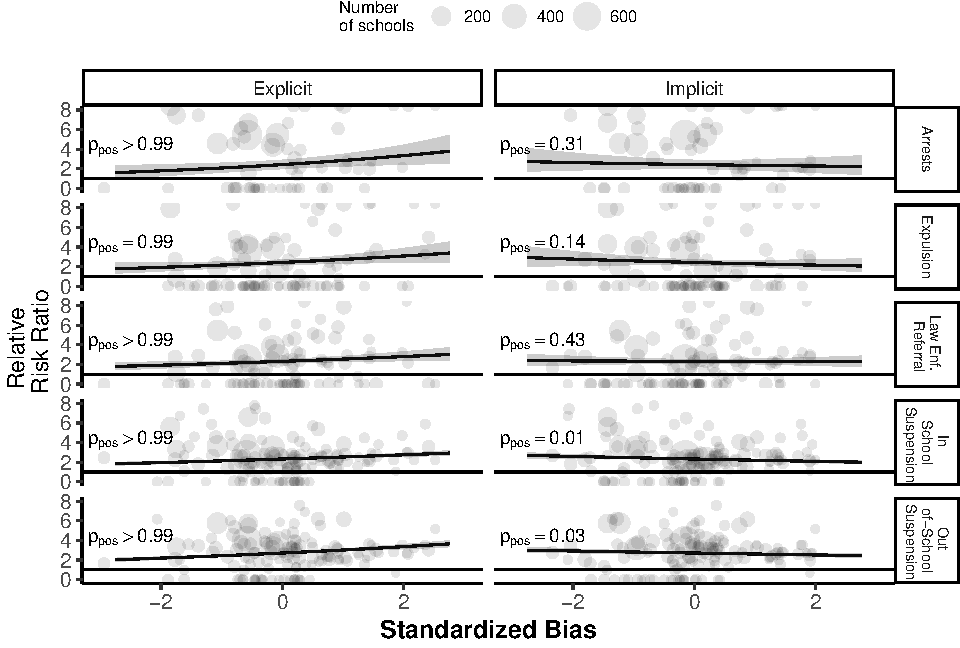
\includegraphics{Riddle_Sinclair_PNAS_files/figure-latex/detail-risks-1.pdf}
\caption{Association between bias and relative risk ratio for black
students to white students. Line is the mean of the posterior. Bands
indicate 95\% uncertainty intervals. Points represent counties, whose
sizes are scaled to the number of schools in that county. Printed
p\_\{pos\} represents the posterior probability that the association is
positive. Note that the y axis is cut at 8 for legibility despite data
extending beyond. Additionally, a number of schools cannot be
represented because the ratio of discipline proportions (black/white) is
undefined, either because there are zero students of a given race
enrolled (e.g.~NA/white), or the proportion of white students
disciplined is zero (e.g.~black/0).}
\end{figure}

To better illustrate the nature of these relationships, figure
@ref(fig:detail-risks) shows the estimated relative risk ratios for each
type of bias measurement and each disciplinary metric. This quantity is
the ratio of the probability that a black student will receive a given
disciplinary action to the probability that a white students will
receive a given disciplinary action. Higher values indicate that black
students have a higher probability of being punished than white
students. Examining the risk ratio for out-of-school suspensions, in a
hypothetical county with 0 standardized bias on both implicit and
explicit, the model predicts that for every white student suspended, we
should expect 2.71 {[}2.65, 2.78{]} black students to be suspended. If
we move to a county one standard deviation above the mean of explicit
bias, the ratio of black to white students suspended increases to 3.02
{[}2.9, 3.14{]}, while the same movement for implicit bias decreases the
ratio to 2.61 {[}2.52, 2.71{]}.

\subsection{Additional analyses: Sexuality bias as
predictor}\label{additional-analyses-sexuality-bias-as-predictor}

We sought to test whether the relationships observed above were specific
to estimates of racial bias. Accordingly, we ran the same set of
analyses with sexuality bias replacing racial bias.

\subsubsection{Project Implicit
Estimates}\label{project-implicit-estimates-1}

The unstandardized county-level estimates of bias adjusted with
poststratification, evidence a pro-straight bias in both implicit
(\(mean\) = 0.38, \(sd\) = 0.05) and explicit measures (\(mean\) = 1.65,
\(sd\) = 0.49), where on both scales 0 = no bias, and positive numbers
indicate a pro-straight bias.

\subsubsection{Associations across
counties}\label{associations-across-counties-1}

Figure @ref(fig:overall-associations-sex) shows the estimate of primary
interest for each of the models. The estimates displayed are the
coefficients for the interaction between race and each of the two bias
measurements. Given that Black Americans are the baseline group,
negative values for this coefficient indicate that as one moves into
counties with higher levels of bias, the gap between the probability of
a black student being disciplined and the probability of a white student
being disciplined grows. Table @ref(tab:reg-coefs-sex) displays the
estimated coefficients and 95\% uncertainty intervals for each of the
fixed effects for each model.

\begin{figure}
\centering
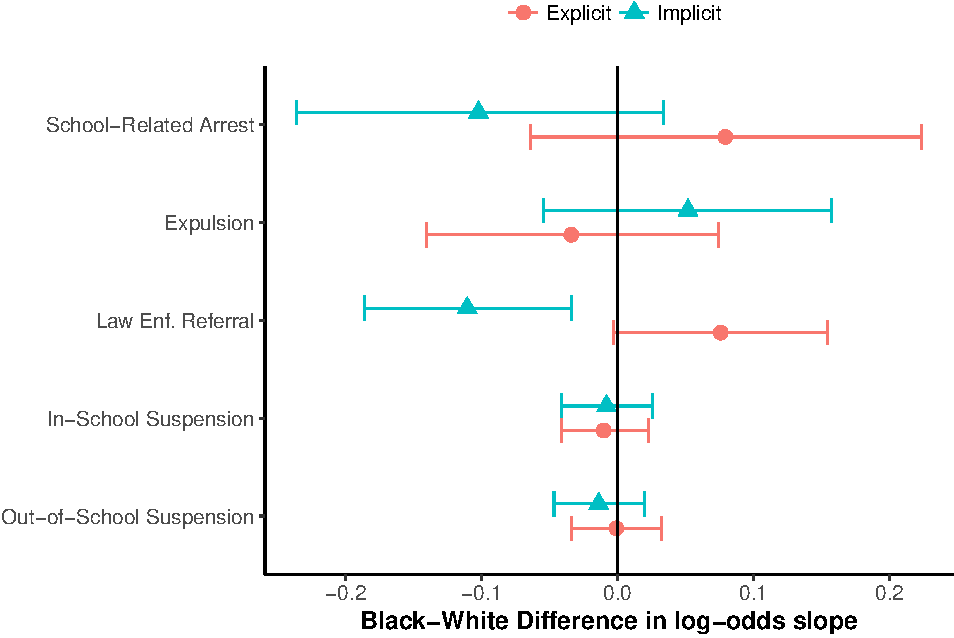
\includegraphics{Riddle_Sinclair_PNAS_files/figure-latex/overall-associations-sex-1.pdf}
\caption{Association between each metric and county-level estimates of
explicit and implicit bias. Negative values indicate that the rate of
increase (or decrease) for blacks is faster (or slower) than for whites.
Point is the mean of the posterior and error bars represent 95\%
bayesian uncertainty intervals.}
\end{figure}

\begin{table}[!htbp] \centering 
  \caption{Regression coefficient estimates for the population-level (i.e. fixed) effects, along with 95\% uncertainty intervals for each of the disciplinary metrics.} 
  \label{tab:reg-coefs-sex} 
\begin{tabular}{@{\extracolsep{5pt}} cccccc} 
\\[-1.8ex]\hline 
\hline \\[-1.8ex] 
 & Out-of-School Suspension & In-School Suspension & Law Enf. Referral & Expulsion & School-Related Arrest \\ 
\hline \\[-1.8ex] 
Intercept & \textbackslash bf\{-2.29\}, [-2.32,-2.26] & \textbackslash bf\{-2.23\}, [-2.27,-2.19] & \textbackslash bf\{-5.72\}, [-5.83,-5.62] & \textbackslash bf\{-6.54\}, [-6.67,-6.41] & \textbackslash bf\{-7.98\}, [-8.2,-7.77] \\ 
black-white ratio & \textbackslash bf\{-0.19\}, [-0.25,-0.14] & \textbackslash bf\{-0.43\}, [-0.51,-0.36] & \textbackslash bf\{0.18\}, [0.03,0.35] & -0.11, [-0.31,0.08] & 0.11, [-0.21,0.44] \\ 
proportion black & \textbackslash bf\{0.33\}, [0.25,0.41] & \textbackslash bf\{0.44\}, [0.34,0.54] & \textbackslash bf\{-0.42\}, [-0.64,-0.2] & -0.16, [-0.42,0.1] & -0.29, [-0.68,0.1] \\ 
college grads & \textbackslash bf\{0.05\}, [0.01,0.09] & \textbackslash bf\{-0.05\}, [-0.1,0] & \textbackslash bf\{0.14\}, [0.02,0.25] & -0.01, [-0.15,0.12] & \textbackslash bf\{0.23\}, [0.04,0.42] \\ 
crime & 0.03, [0,0.06] & \textbackslash bf\{0.06\}, [0.02,0.1] & 0.03, [-0.05,0.12] & \textbackslash bf\{0.14\}, [0.04,0.24] & 0.03, [-0.11,0.18] \\ 
housing density & \textbackslash bf\{-0.04\}, [-0.07,-0.02] & -0.03, [-0.06,0.01] & 0, [-0.07,0.06] & -0.05, [-0.13,0.03] & \textbackslash bf\{-0.14\}, [-0.24,-0.04] \\ 
dissimilarity & \textbackslash bf\{0.17\}, [0.14,0.21] & \textbackslash bf\{0.09\}, [0.05,0.13] & \textbackslash bf\{0.17\}, [0.07,0.27] & \textbackslash bf\{0.29\}, [0.17,0.41] & \textbackslash bf\{0.48\}, [0.31,0.66] \\ 
income & \textbackslash bf\{-0.08\}, [-0.13,-0.03] & -0.03, [-0.09,0.04] & -0.07, [-0.2,0.07] & \textbackslash bf\{-0.27\}, [-0.43,-0.1] & 0.01, [-0.21,0.24] \\ 
mobility & \textbackslash bf\{-0.05\}, [-0.09,-0.02] & -0.03, [-0.07,0.02] & 0.09, [-0.02,0.2] & -0.01, [-0.16,0.14] & 0, [-0.21,0.2] \\ 
poverty & -0.02, [-0.1,0.06] & \textbackslash bf\{0.15\}, [0.05,0.25] & \textbackslash bf\{-0.46\}, [-0.69,-0.23] & \textbackslash bf\{-0.38\}, [-0.66,-0.09] & -0.3, [-0.68,0.08] \\ 
total population & -0.01, [-0.04,0.01] & -0.02, [-0.06,0.01] & -0.03, [-0.11,0.04] & 0, [-0.08,0.08] & \textbackslash bf\{0.11\}, [0.01,0.22] \\ 
unemployment & \textbackslash bf\{0.2\}, [0.16,0.24] & 0.04, [-0.01,0.09] & 0.09, [-0.03,0.2] & \textbackslash bf\{0.21\}, [0.06,0.35] & 0.15, [-0.06,0.36] \\ 
proportion white & 0.03, [-0.04,0.1] & \textbackslash bf\{0.09\}, [0,0.18] & \textbackslash bf\{-0.23\}, [-0.43,-0.04] & -0.23, [-0.47,0.02] & -0.15, [-0.49,0.18] \\ 
race: white & \textbackslash bf\{-1.06\}, [-1.09,-1.03] & \textbackslash bf\{-0.91\}, [-0.93,-0.88] & \textbackslash bf\{-0.86\}, [-0.94,-0.77] & \textbackslash bf\{-0.88\}, [-0.99,-0.76] & \textbackslash bf\{-0.89\}, [-1.08,-0.7] \\ 
implicit bias & \textbackslash bf\{0.05\}, [0,0.09] & \textbackslash bf\{0.13\}, [0.07,0.19] & 0.02, [-0.1,0.14] & \textbackslash bf\{0.2\}, [0.05,0.35] & \textbackslash bf\{0.4\}, [0.18,0.61] \\ 
explicit bias & \textbackslash bf\{-0.14\}, [-0.19,-0.1] & -0.03, [-0.08,0.03] & \textbackslash bf\{-0.26\}, [-0.38,-0.15] & -0.15, [-0.29,0] & \textbackslash bf\{-0.36\}, [-0.57,-0.14] \\ 
black-white ratio\textasteriskcentered race: white & \textbackslash bf\{0.13\}, [0.08,0.18] & 0.06, [0,0.12] & \textbackslash bf\{-0.22\}, [-0.43,-0.02] & 0.16, [-0.05,0.36] & -0.2, [-0.6,0.17] \\ 
proportion black\textasteriskcentered race: white & \textbackslash bf\{-0.09\}, [-0.16,-0.03] & -0.05, [-0.12,0.01] & 0.13, [-0.05,0.3] & -0.06, [-0.28,0.16] & 0.12, [-0.21,0.45] \\ 
college grads\textasteriskcentered race: white & \textbackslash bf\{-0.12\}, [-0.15,-0.09] & \textbackslash bf\{-0.06\}, [-0.09,-0.02] & \textbackslash bf\{-0.18\}, [-0.25,-0.1] & \textbackslash bf\{-0.13\}, [-0.24,-0.02] & -0.09, [-0.23,0.06] \\ 
crime\textasteriskcentered race: white & -0.02, [-0.04,0] & 0.01, [-0.02,0.03] & 0.02, [-0.03,0.07] & -0.04, [-0.1,0.03] & 0.05, [-0.04,0.14] \\ 
housing density\textasteriskcentered race: white & \textbackslash bf\{-0.02\}, [-0.04,0] & -0.01, [-0.03,0.01] & -0.01, [-0.04,0.02] & -0.03, [-0.08,0.02] & -0.06, [-0.22,0.09] \\ 
dissimilarity\textasteriskcentered race: white & \textbackslash bf\{-0.11\}, [-0.14,-0.08] & \textbackslash bf\{-0.05\}, [-0.08,-0.02] & \textbackslash bf\{-0.09\}, [-0.16,-0.02] & -0.04, [-0.13,0.05] & \textbackslash bf\{-0.2\}, [-0.33,-0.08] \\ 
income\textasteriskcentered race: white & \textbackslash bf\{-0.06\}, [-0.09,-0.02] & \textbackslash bf\{-0.09\}, [-0.13,-0.05] & -0.06, [-0.15,0.02] & 0.03, [-0.1,0.17] & -0.1, [-0.25,0.05] \\ 
mobility\textasteriskcentered race: white & 0.03, [0,0.07] & 0.01, [-0.03,0.04] & -0.04, [-0.13,0.04] & -0.01, [-0.13,0.12] & 0.05, [-0.12,0.22] \\ 
poverty\textasteriskcentered race: white & 0.05, [-0.02,0.11] & 0, [-0.07,0.06] & -0.09, [-0.25,0.07] & 0.02, [-0.21,0.24] & -0.05, [-0.33,0.23] \\ 
total population\textasteriskcentered race: white & \textbackslash bf\{-0.03\}, [-0.05,-0.01] & -0.01, [-0.03,0.01] & 0, [-0.04,0.03] & -0.02, [-0.06,0.03] & -0.01, [-0.05,0.04] \\ 
unemployment\textasteriskcentered race: white & 0, [-0.03,0.03] & 0.01, [-0.02,0.04] & -0.02, [-0.1,0.06] & 0.04, [-0.06,0.15] & -0.01, [-0.16,0.14] \\ 
proportion white\textasteriskcentered race: white & 0.01, [-0.04,0.07] & 0.01, [-0.05,0.06] & -0.1, [-0.23,0.02] & 0.06, [-0.13,0.24] & -0.07, [-0.29,0.14] \\ 
implicit bias\textasteriskcentered race: white & -0.01, [-0.05,0.02] & -0.01, [-0.04,0.02] & \textbackslash bf\{-0.11\}, [-0.19,-0.04] & 0.05, [-0.05,0.16] & -0.1, [-0.24,0.03] \\ 
explicit bias\textasteriskcentered race: white & 0, [-0.03,0.03] & -0.01, [-0.04,0.02] & 0.08, [0,0.15] & -0.03, [-0.14,0.07] & 0.08, [-0.07,0.23] \\ 
\hline \\[-1.8ex] 
\end{tabular} 
\end{table}

This figure illustrates that in general, county-level explicit and
implicit biases in favor of straight individuals are not consistently
associated with racial disciplinary disparities. The one exception is
for law enforcement referrals, where we see that counties with higher
levels of implicit bias are expected to have a larger racial gap
(\(M_{slope}\) = -0.11, {[}-0.19, -0.03{]}). For this particular
disciplinar action, explicit biases tend to show the opposite
association, with counties higher in explicit bias expected to have a
smaller racial gap, though the evidence is not as conclusive
(\(M_{slope}\) = 0.08, {[}0, 0.15{]}). All other estimates are located
near zero, or are inconclusive with respect to the direction of the
effect.

\section{Discussion}\label{discussion}

These analyses across five types of disciplinary actions are fully
consistent with county-level estimates of explicit racial bias being
associated with racial disciplinary disparities. Specifically, in
counties where the white population is estimated to have higher rates of
explicit biases that favor whites, the difference in suspensions,
expulsions, law enforcement referrals, and school-related arrests
between black and white students is expected to be greater than in those
counties where the white population has lower rates of explicit racial
biases. In a secondary set of analyses with sexuality bias, we found
evidence that the aforementioned pattern cannot be explained by a more
general tendency to exhibit explicit biases to stigmatized groups, as
opposed to racial biases specifically, since most of the associations
with respect to county-level explicit and implicit sexuality bias are
directionally inconclusive. Additionally, our analyses cover the vast
majority of school-aged students in the United States, and our models
include a large set of covariates, suggesting that the relationships
observed are not attributable to other indicators that can often
co-occur with racial disparities, such as socioeconomic status or
population demographics (10, 31).

Of course, this research is not without limitations and anomalies. The
relationship between implicit racial bias and suspension was in an
unexpected direction. That is, greater implicit bias is somewhat
associated with smaller racial disparities in suspensions. One
possibility is that counties higher in implicit bias are not as likely
to suspend black students, but rather opt to use other disciplinary
tools unmeasured in these data. Another possibility is that people in
counties characterized by higher implicit bias are somewhat willing and
able to correct their behavioral responses in order to conform to their
egalitarian explicit beliefs or egalitarian social norms {[}(32). Much
research at the individual level shows that people are able to
counteract the automatic impulses associated with implicit bias when
they have the motivation and cognitive bandwidth to do so (33).
Additionally, because of the correlational nature of the analyses, it is
impossible to definitively establish the causal relationship between
explicit bias and disciplinary disparities. The conclusion that explicit
biases predict disciplinary disparities is consonant with a great deal
of research on disciplinary disparities {[}(34). However, it is also
possible that living in a region in which black students are disciplined
to a greater extent than white students exacerbates and/or reinforces
the explicit racial biases of community members, or that the
relationship between explicit racial biases and disciplinary disparities
is bi-directional. Finally, although we used a poststratification scheme
to make our estimates more representative with respect to county age
distributions, we cannot account for other ways in which Project
Implicit data are not representative of the general population. Our
analyses trade off the ability to ask these more detailed question with
the strengths of statistical power and population coverage offered by
the large datasets we used here. A full understanding of the complex
issues shaping racial disciplinary disparities will require integrating
findings from carefully controlled experiments, targeted surveys,
administrative databases, and large-scale observational data.

Nevertheless, our work compliments other research indicating that racial
dynamics are an important source for the observed differences in
disciplinary rates between black and white students. For instance,
students, caregivers, and administrators perceive suspensions and the
disproportionate use of them as at least partially racially motivated
(35--37). Additionally, other work has shown that even after controlling
for a range of other factors, race remains associated with the
likelihood of receiving disciplinary actions (10, 29). Additionally,
experimental evidence shows that disciplinary decision-making for
teachers differs depending on the race of the student (11). The present
research adds to this work by showing for the first time associations
between disciplinary actions and measurements of racial bias.

Our work also compliments existing studies examining the degree to which
implicit and explicit racial biases are associated with racial
disparities in key areas, such as health and policing (14--16) by
extending this type of inquiry to educational outcomes. To properly
assess the meaning of these findings, it is imperative that future work
focus specifically on what it means to exist in a community that is
estimated to have high or low levels of implicit or explicit bias.

As we have already highlighted, students who are subject to the
disciplinary actions we examined here are at substantially higher risk
for negative life outcomes (8). In dispensing these disciplinary
decisions differentially across racial groups, educational agencies are
also differentially allocating life prospects. Although implementing
training and education focused on implicit bias is popular among
educational administrators (38), and has been recommended by the US
Department of Education (39), our analysis suggests that effectively
combating racial disparities in discipline requires confronting more
explicit forms of racial bias, perhaps, for example, through peer
influence or interventions designed to change social norms (40).

We offer the research presented here to prompt additional scrutiny with
respect to how and why educational agencies in the United States
differentially administer disciplinary actions, especially when those
actions are known to have dire consequences for student welfare.
Although the focus here is on actions taking place within educational
agencies, the mechanisms responsible for these disparities likely exist,
at least partly, in the larger community. Through understanding and
reducing these disciplinary disparities specifically and the biases that
exist in the community more broadly, there exists an avenue for
education to maximize its promise as the great equalizer it has the
potential to be.

\subsection{Materials \& Methods}\label{materials-methods}

\subsubsection{Analytic Approach}\label{analytic-approach}

Because Project Implicit is a nonrandom sample, we used multilevel
regression and post-stratification to obtain accurate geographical
population-based estimates of implicit and explicit bias. This procedure
corrects for biased sampling and regularizes extreme observations with
little data to support them (e.g.~a county with only a handful of
respondents with especially high or low scores) (41, 42). Following past
work (14), we identified age as one dimension along which IAT
respondents differed from the general population in ways that could bias
our conclusions (43). Our post-stratification weighting scheme is as
follows: We first grouped respondents into five age group categories
(15-24, 25-34, 35-54, 55-75, and 75+). We next fit multilevel models
estimating bias (implicit and explicit biases separately) as a function
of our state-level covariates (the ``fixed'' effects: all identical to
those included in the final model, described below), and allowed the
estimates to vary by age bin, county, and state (the ``random''
effects). Next, we determined the population of whites in each county in
these age groups using the American Community Survey's 5-year estimates
ending in 2014. Finally, we used our estimated models to predict the
expected response for each age bin, in each county. Our final
county-level estimates are the average of the values predicted for the 5
age bins, weighted by the population size of that bin in that county. As
a result of this procedure, we can be confident that our county-level
estimates should more closely approximate what our estimates would look
like if the Project Implicit data were truly representative along the
age dimension in all counties.

We analyzed these data using a series of bayesian multilevel logistic
regressions. We modeled the probability that a student would be expelled
as a function of a set of effects that are constant across observations
(i.e.~fixed effects: race (dummy coded), implicit bias, explicit bias,
an interaction term between race and implicit bias, an interaction term
between race and explicit bias, and all covariates described below, plus
each of the covariates interacting with race) and a set of effects that
vary across counties (i.e.~random effects: overall intercept \& race).
We fit separate models for each of the outcomes. All numerical
predictors were standardized at the appropriate level (county, state)
before model estimation (for post-stratification as well as for final
inference) to help with estimation efficiency and interpretability. We
also set priors for the intercept and coefficients in the bayesian model
to be weakly informative normal distributions centered on zero with a
standard deviation of five. This corresponds to a prior belief that all
parameters take values between -15 and 15 with a probability of more
than .99. Realistically, values outside this range are extremely
unlikely given that all variables were standardized prior to estimation.
Priors on all other parameters (e.g.~variance of the county-level
intercepts) were left to default settings from the software package used
to fit the models.

Because of the computational demands of fitting such a high-dimensional
model to such a large dataset (the full model for each metric would
consist of over 6k parameters to approximately 170k observations), we
used a consensus monte carlo algorithm to obtain approximate posterior
distributions for the parameters of interest (44). The approximate
posteriors derived from this algorithm have been shown to be nearly
indistinguishable from the true posterior, a result we verified using a
small subset of our own data. \#\#\# Data Sources \#\#\#\# Disciplinary
actions

To assess rates of disciplinary action, we used data from the Civil
Rights Data Collection (CRDC) conducted by the US Department of
Education. The dataset we used comes from the 2013-2014 academic year
and has data on ``all public local and educational agencies and schools,
including long-term secure juvenile justice facilities, charter schools,
alternative schools, and schools serving students with disabilities.''
In total, the CRDC data represents 95507 institutions enrolling
approximately 50 million students, of which approximately 25.2 million
are white and 7.8 million are Black\footnote{We note that we initially
  preregistered a number of analyses concerning this work. There are a
  number of differences between the analyses we registered and those
  presented in the main text. The registered analyses can be found, in
  full, in the project's OSF page (\url{https://osf.io/pu79a/}).}.
Previous work using CRDC data have identified a number of districts
whose data are in error, and have excluded juvenile justice facilities,
as these institutions constitute dramatically different educational
environments, where the meaning of disciplinary actions may be quite
different (45). We followed similar practices, excluding all juvenile
justice facilities. Additionally, we excluded data for a specific
disciplinary metric for any schools which reported disciplining more
students than it reported enrolling for \emph{any} race for that metric
(e.g.~a school reported expelling 5 white students when they reported
enrolling less than that number). We also excluded any school for all
disciplinary actions if they had an overreporting error for 3 or more
metrics. After these exclusions are applied, the final sample used for
modeling consists of 93493 institutions, enrolling 49.8 million students
of which 25.1 million are white and 7.7 million are black.\footnote{Researchers
  who compared individual schools' out-of-school suspension rates
  reported in the 2011-2012 CRDC with suspension rates of the same
  schools as reported on state websites where available found a number
  of mismatches (45). We did not have the resources to conduct similar
  comparisons for all outcomes in all 93493 institutions; however,
  informal inspection of the data led us to find one school district for
  which this was the case. Including versus excluding schools from this
  district do not change the results in any meaningful way. The analyses
  presented herein include this district. The results of corresponding
  analyses without this district can be requested from the first author.
  It should be noted that the United States Government Accountability
  Office's recent descriptive overview of the 2013-2014 CRDC also did
  not exclude cases for which there was a discrepancy between
  disciplinary rates reported in this dataset and any disciplinary data
  reported on state websites(46). As such, the analyses here are
  consistent with the only other published examination of the 2013-2014
  CRDC data that we are aware of.} From these data, we focus on the
number of students by race (black and white) who were subjected to each
of the disciplinary actions described below.

\subparagraph{Types of disciplinary
actions}\label{types-of-disciplinary-actions}

We report here on five different types of disciplinary actions:
in-school suspensions, out-of-school suspensions, law enforcement
referrals, school-related arrests, and expulsions.

The most extreme outcome, \emph{expulsion}, is defined as when a student
is prohibited from returning to the educational institution for the
remainder of the school year or longer. The institution may or may not
set up alternative educational services for the student. \emph{Law
enforcement referrals} are actions where a student is ``reported to any
law enforcement agency or official for an incident including a school
police unit, for an incident that occurs on school grounds, during
school-related events, or while taking school transportation, regardless
of whether official action is taken. Citations, tickets, and court
referrals are considered referrals to law enforcement.''
\emph{School-related arrests} refer to ``an arrest of a student for any
activity conducted on school grounds, during off-campus school
activities (including while taking school transportation)''
\emph{Out-of-school suspensions} are actions where the student ``is
temporarily removed from his or her regular school for at least half a
day (but less than the remainder of the school year)''. Finally,
\emph{in-school suspensions} are actions where the student is
``temporarily removed from his or her regular classroom(s) for at least
half a day\ldots{},but remains under the direct supervision of school
personnel. Direct supervision means school personnel are physically in
the same location as the student under their supervision.'' (47)

\paragraph{Racial Bias}\label{racial-bias}

We used measurements of implicit and explicit bias available from data
collected through Project Implicit (30). For a full description of the
implicit and explicit bias measures available in these data, refer to
(30) and (14). We note only that we used the IAT D-score as a measure of
implicit bias, and the difference between reported warmth towards whites
and warmth towards black (both measured from 0=very cold to 10=very
warm) as a measure of explicit bias. Additionally, we used only
respondents who had geographic information that would allow us to place
them in a United States county, identified as White, and visited the
site anytime after it went live in 2002 through the end of 2014. This
consisted of approximately 1.3 million total respondents from 3099
counties. 1.19 million respondents provided data for the IAT, and 1.15
million provided explicit bias ratings.

\paragraph{Sexuality Bias}\label{sexuality-bias}

We used measurements of implicit and explicit sexuality bias available
from data collected through Project Implicit (30). We opted for these
measures as robustness checks because there were enough observations to
closely mimic the racial bias analyses, and they have been used for
similar purposes in previous work (15) As in the previous study, we used
the IAT D-score as a measure of implicit bias. Our warmth score
represented the average of the difference between straight men and gay
men and the difference between straight women and lesbian women. We used
only respondents who had geographic information that would allow us to
place them in a United States county and visited the anytime between
when it went live in 2002 through the end of 2014. This consisted of
approximately 798K total respondents from 3044 counties. Of these
respondents, 720K respondents provided data for the IAT, and 761K
respondents provided explicit bias ratings.

\paragraph{Covariates}\label{covariates}

Each county-level variable used as a covariate in the final model and
the corresponding state-level variable used as a predictor in the
post-stratification scheme (described below) were taken from the same
source. Population size and proportions, socioeconomic indicators,
mobility, and segregation indices were all taken from the American
Community Survey (ACS) 5-year estimates for the time period ending in
2014. Urban-rural indicators were taken from the 2010 US Census, and
crime rates were taken from the FBI Uniform Crime Reporting program, as
made available through the National Archive of Criminal Justice Data for
each year from 2010-2014\footnote{These years are chosen to for the FBI
  data to yield estimates that are similar to the 5-year estimates from
  the ACS data.}. Each of these variables is described below.

\subparagraph{Population size and
proportions}\label{population-size-and-proportions}

We obtained the total population, the proportion of the population that
is white, the proportion of the population that is black, and the ratio
of black-to-white people in the population from ACS table B02001.

\subparagraph{Socioeconomic indicators}\label{socioeconomic-indicators}

We obtained estimates for the percentage of population with a Bachelor's
degree or higher, the percentage of the population aged 16 or over in
the labor force that is unemployed, the median household income, and the
percentage of families and people whose income in the last year was
below the poverty line from the ACS table DP03.

\subparagraph{Urban-rural indicator}\label{urban-rural-indicator}

We obtained estimates of housing density per square mile of land area
from Census table GCT-PH1.

\subparagraph{Mobility}\label{mobility}

We obtained estimates of population mobility by summing the percentage
of Black Americans who moved from a different county, state, or country
into the county of interest (county-level covariate) or who moved from a
different state or country into the state of interest (state-level
covariate). We took these metrics from the ACS table S0701.

\subparagraph{Crime}\label{crime}

We computed estimates of the number of violent crimes per person by
taking the number of crimes reported divided by the population size for
each year, and averaging the resulting proportions across the 5 years of
data.

\subparagraph{Segregation}\label{segregation}

We computed a dissimiliarity index as described by (48). This metric is
computed based on the racial dissimilarity of census tracts within a
county, and reflects the proportion of a group within the county that
would have to move in order for all census tracts to have group
distributions that matched the overall distribution of the county. These
computations were done using data from the ACS table B02001.

\showmatmethods
\showacknow
\pnasbreak

\hypertarget{refs}{}
\hypertarget{ref-kinsler2011understanding}{}
1. Kinsler J (2011) Understanding the black--white school discipline
gap. \emph{Economics of Education Review} 30(6):1370--1383.

\hypertarget{ref-okonofua2016vicious}{}
2. Okonofua JA, Walton GM, Eberhardt JL (2016) A vicious cycle: A
social--psychological account of extreme racial disparities in school
discipline. \emph{Perspectives on psychological science} 11(3):381--398.

\hypertarget{ref-aud2011america}{}
3. Aud S, KewalRamani A, Frohlich L (2011) America's youth: Transitions
to adulthood. nces 2012-026. \emph{National Center for Education
Statistics}.

\hypertarget{ref-yeager2017loss}{}
4. Yeager DS, Purdie-Vaughns V, Hooper SY, Cohen GL (2017) Loss of
institutional trust among racial and ethnic minority adolescents: A
consequence of procedural injustice and a cause of life-span outcomes.
\emph{Child development} 88(2):658--676.

\hypertarget{ref-gregory1995crime}{}
5. Gregory JF (1995) The crime of punishment: Racial and gender
disparities in the use of corporal punishment in us public schools.
\emph{Journal of Negro Education}:454--462.

\hypertarget{ref-skiba2011race}{}
6. Skiba RJ, et al. (2011) Race is not neutral: A national investigation
of african american and latino disproportionality in school discipline.
\emph{School Psychology Review} 40(1):85.

\hypertarget{ref-pager2009sequencing}{}
7. Pager D, Western B, Sugie N (2009) Sequencing disadvantage: Barriers
to employment facing young black and white men with criminal records.
\emph{The ANNALS of the American Academy of Political and Social
Science} 623(1):195--213.

\hypertarget{ref-hirschfield2009another}{}
8. Hirschfield P (2009) Another way out: The impact of juvenile arrests
on high school dropout. \emph{Sociology of Education} 82(4):368--393.

\hypertarget{ref-togut2011gestalt}{}
9. Togut TD (2011) The gestalt of the school-to-prison pipeline: The
duality of overrepresentation of minorities in special education and
racial disparity in school discipline eon minorities. \emph{American
University Journal of Gender, Social Policy \& the Law} 20:163.

\hypertarget{ref-skiba2002color}{}
10. Skiba RJ, Michael RS, Nardo AC, Peterson RL (2002) The color of
discipline: Sources of racial and gender disproportionality in school
punishment. \emph{The urban review} 34(4):317--342.

\hypertarget{ref-okonofua2015two}{}
11. Okonofua JA, Eberhardt JL (2015) Two strikes: Race and the
disciplining of young students. \emph{Psychological science}
26(5):617--624.

\hypertarget{ref-gregory2008discipline}{}
12. Gregory A, Weinstein RS (2008) The discipline gap and african
americans: Defiance or cooperation in the high school classroom.
\emph{Journal of School Psychology} 46(4):455--475.

\hypertarget{ref-rudman2004sources}{}
13. Rudman LA (2004) Sources of implicit attitudes. \emph{Current
Directions in Psychological Science} 13(2):79--82.

\hypertarget{ref-leitner2016blacks}{}
14. Leitner JB, Hehman E, Ayduk O, Mendoza-Denton R (2016) Blacks' death
rate due to circulatory diseases is positively related to whites'
explicit racial bias: A nationwide investigation using project implicit.
\emph{Psychological science} 27(10):1299--1311.

\hypertarget{ref-orchard2017county}{}
15. Orchard J, Price J (2017) County-level racial prejudice and the
black-white gap in infant health outcomes. \emph{Social Science \&
Medicine} 181:191--198.

\hypertarget{ref-hehman2017disproportionate}{}
16. Hehman E, Flake JK, Calanchini J (2017) Disproportionate use of
lethal force in policing is associated with regional racial biases of
residents. \emph{Social Psychological and Personality
Science}:1948550617711229.

\hypertarget{ref-verdugo2002race}{}
17. Verdugo RR (2002) Race-ethnicity, social class, and zero-tolerance
policies: The cultural and structural wars. \emph{Education and urban
society} 35(1):50--75.

\hypertarget{ref-cadinu2003stereotype}{}
18. Cadinu M, Maass A, Frigerio S, Impagliazzo L, Latinotti S (2003)
Stereotype threat: The effect of expectancy on performance.
\emph{European Journal of Social Psychology} 33(2):267--285.

\hypertarget{ref-darley1980expectancy}{}
19. Darley JM, Fazio RH (1980) Expectancy confirmation processes arising
in the social interaction sequence. \emph{American psychologist}
35(10):867.

\hypertarget{ref-major2005social}{}
20. Major B, O'brien LT (2005) The social psychology of stigma.
\emph{Annu Rev Psychol} 56:393--421.

\hypertarget{ref-jetten1996intergroup}{}
21. Jetten J, Spears R, Manstead AS (1996) Intergroup norms and
intergroup discrimination: Distinctive self-categorization and social
identity effects. \emph{Journal of personality and social psychology}
71(6):1222.

\hypertarget{ref-pettigrew1958personality}{}
22. Pettigrew TF (1958) Personality and sociocultural factors in
intergroup attitudes: A cross-national comparison. \emph{Journal of
conflict resolution} 2(1):29--42.

\hypertarget{ref-payne2017bias}{}
23. Payne BK, Vuletich HA, Lundberg KB (2017) The bias of crowds: How
implicit bias bridges personal and systemic prejudice.
\emph{Psychological Inquiry} 28(4):233--248.

\hypertarget{ref-markus2010cultures}{}
24. Markus HR, Kitayama S (2010) Cultures and selves: A cycle of mutual
constitution. \emph{Perspectives on psychological science}
5(4):420--430.

\hypertarget{ref-cuellar2015school}{}
25. Cuellar AE, Markowitz S (2015) School suspension and the
school-to-prison pipeline. \emph{International Review of Law and
Economics} 43:98--106.

\hypertarget{ref-matjasko2011effective}{}
26. Matjasko JL (2011) How effective are severe disciplinary policies?
School policies and offending from adolescence into young adulthood.
\emph{Journal of school psychology} 49(5):555--572.

\hypertarget{ref-rausch2005academic}{}
27. Rausch MK, Skiba RJ, Simmons A (2005) The academic cost of
discipline: The relationship between suspension/expulsion and school
achievement. \emph{Annual Meeting of the American Educational Research
Association, Montreal, Canada}.

\hypertarget{ref-hemphill2006effect}{}
28. Hemphill SA, Toumbourou JW, Herrenkohl TI, McMorris BJ, Catalano RF
(2006) The effect of school suspensions and arrests on subsequent
adolescent antisocial behavior in australia and the united states.
\emph{Journal of Adolescent Health} 39(5):736--744.

\hypertarget{ref-anyon2014persistent}{}
29. Anyon Y, et al. (2014) The persistent effect of race and the promise
of alternatives to suspension in school discipline outcomes.
\emph{Children and Youth Services Review} 44:379--386.

\hypertarget{ref-xu2014psychology}{}
30. Xu K, Nosek B, Greenwald A (2014) Psychology data from the race
implicit association test on the project implicit demo website.
\emph{Journal of Open Psychology Data} 2(1).

\hypertarget{ref-williams1999race}{}
31. Williams DR (1999) Race, socioeconomic status, and health the added
effects of racism and discrimination. \emph{Annals of the New York
Academy of Sciences} 896(1):173--188.

\hypertarget{ref-pryor2004dual}{}
32. Pryor JB, Reeder GD, Yeadon C, Hesson-McInnis M (2004) A
dual-process model of reactions to perceived stigma. \emph{Journal of
personality and social psychology} 87(4):436.

\hypertarget{ref-devine2002regulation}{}
33. Devine PG, Plant EA, Amodio DM, Harmon-Jones E, Vance SL (2002) The
regulation of explicit and implicit race bias: The role of motivations
to respond without prejudice. \emph{Journal of personality and social
psychology} 82(5):835.

\hypertarget{ref-mcintosh2014education}{}
34. McIntosh K, Girvan EJ, Horner RH, Smolkowski K (2014) Education not
incarceration: A conceptual model for reducing racial and ethnic
disproportionality in school discipline. \emph{Journal of Applied
Research on Children: Informing Policy for Children at Risk} 5(2):4.

\hypertarget{ref-haight2014ecological}{}
35. Haight W, Gibson PA, Kayama M, Marshall JM, Wilson R (2014) An
ecological-systems inquiry into racial disproportionalities in
out-of-school suspensions from youth, caregiver and educator
perspectives. \emph{Children and Youth Services Review} 46:128--138.

\hypertarget{ref-gibson2013caregivers}{}
36. Gibson PA, Haight W (2013) Caregivers' moral narratives of their
african american children's out-of-school suspensions: Implications for
effective family--school collaborations. \emph{Social work}
58(3):263--272.

\hypertarget{ref-ruck2002racial}{}
37. Ruck MD, Wortley S (2002) Racial and ethnic minority high school
students' perceptions of school disciplinary practices: A look at some
canadian findings. \emph{Journal of Youth and Adolescence}
31(3):185--195.

\hypertarget{ref-staats2016understanding}{}
38. Staats C (2016) Understanding implicit bias: What educators should
know. \emph{American Educator} 39(4):29.

\hypertarget{ref-us2014dear}{}
39. US Department of Education \& US Department of Justice (2014)
\emph{Dear colleague letter on the nondiscriminatory administration of
school discipline} (US Department of Education, Office for Civil Rights;
US Department of Justice Washington, DC) Available at:
\url{https://www2.ed.gov/about/offices/list/ocr/letters/colleague-201401-title-vi.pdf}.

\hypertarget{ref-paluck2009prejudice}{}
40. Paluck EL, Green DP (2009) Prejudice reduction: What works? A review
and assessment of research and practice. \emph{Annual review of
psychology} 60:339--367.

\hypertarget{ref-park2004bayesian}{}
41. Park DK, Gelman A, Bafumi J (2004) Bayesian multilevel estimation
with poststratification: State-level estimates from national polls.
\emph{Political Analysis} 12(4):375--385.

\hypertarget{ref-gelman1997poststratification}{}
42. Gelman A, Little TC (1997) Poststratification into many categories
using hierarchical logistic regression. \emph{Survey Methodology}
23(2):127--35.

\hypertarget{ref-gonsalkorale2009aging}{}
43. Gonsalkorale K, Sherman JW, Klauer KC (2009) Aging and prejudice:
Diminished regulation of automatic race bias among older adults.
\emph{Journal of Experimental Social Psychology} 45(2):410--414.

\hypertarget{ref-scott2016bayes}{}
44. Scott SL, et al. (2016) Bayes and big data: The consensus monte
carlo algorithm. \emph{International Journal of Management Science and
Engineering Management} 11(2):78--88.

\hypertarget{ref-losen2015we}{}
45. Losen DJ, et al. (2015) Are we closing the school discipline gap?

\hypertarget{ref-usgao2018discipline}{}
46. United States Government Accountability Office (2018)
\emph{Discipline disparities for black students, boys, and students with
disabilities} Available at:
\url{https://www.gao.gov/assets/700/690828.pdf}.

\hypertarget{ref-crdc2013survey}{}
47. CRDC Survey (2014) 2013-2014 civil rights data collection survey.
Available at:
\href{/url\%7Bhttp://www2.ed.gov/about/offices/list/ocr/docs/crdc-2013-14-p1-p4.doc\%7D}{\textbackslash{}url\{http://www2.ed.gov/about/offices/list/ocr/docs/crdc-2013-14-p1-p4.doc\}}.

\hypertarget{ref-massey1988dimensions}{}
48. Massey DS, Denton NA (1988) The dimensions of residential
segregation. \emph{Social forces} 67(2):281--315.



% Bibliography
% \bibliography{pnas-sample}

\end{document}

